
\section{Tests Unitaires}
\label{tests:unitaires}

\subsection{Module SQLite}
\label{tests:unitaires:sqlite}

\subsubsection{Sélection aléatoire}
\label{tests:unitaires:sqlite:random}

Ce test unitaire vérifie que deux sélections totalement aléatoires (toutes les
options non renseignées) sont bien différentes, comme demandé dans la
spécification. Son déroulement est assez simple, on réalise deux sélections avec
une liste d'options vide, puis on compare les deux ensembles sélectionnés.
Pour cela on cherche les pistes du premier ensemble sélectionné dans le second
ensemble. Si un élément du premier ensemble n'est pas présent dans le second,
les ensemble sont différents et le test est réussi.

\subsubsection{Filtrage par année}
\label{tests:unitaires:sqlite:annee}

Ce test vérifie que le filtrage des morceau par année fonctionne. Il choisit les
années de sélection entre 1990 et 2000, car c'est une période suffisamment
présente dans la MSD. Ensuite il faut analyser les pistes de l'ensemble
sélectionné et vérifier que leur année de sortie est bien comprise dans
l'intervalle d'années précisée. Si tous les morceaux passent ce test, le test
est une réussite.

\subsubsection{Filtrage par popularité}
\label{tests:unitaires:sqlite:popularite}

Ce test vérifie si le filtrage par popularité fonctionne. La popularité choisie 
pour la sélection est de 0.8, car c'est le seuil à partir duquel les artistes
assez connus apparaissent. Après la sélection, on vérifie si tous les morceaux
de l'ensemble sélectionné on une popularité correspondante au facteur de
filtrage. Si tous les morceaux ont une popularité valide, le test est une
réussite.

\section{Tests de qualité de la playlist}
\label{tests:qualite}


La qualité d'une playlist est très subjective. Cependant dans notre projet cette
qualité est assuré par notre algorithme de similarité. Il fallait donc des tests
pour attester de la qualité de cette similarité. Les test qui vont suivre
\footnote{Ces test n'ont pas pu être implémentés faute de temps, mais nous
pensions qu'il était intéressant de noter leur méthodologie} ne sont pas des
test binaires (seulement réussit ou raté), mais des outils permettant d'analyser 
la qualité d'un algorithme de similarité.

\subsection{Test de cohérence : Technique du «~Grand Fossé~»}
\label{tests:qualite:coherence-fosse}

Ce test permet de tester la \emph{cohérence} de la playlist. Il repose sur la
génération de deux ensembles de morceaux très différents qui constitueront les
données dans lesquelles les morceaux seront sélectionnées, On crée donc
artificiellement un «~fossé~» entre les morceaux. On n'utilise donc pas la
«~vraie~» base de données. Nous avons choisit de simuler deux ensembles très
différents selon les critères suivant~:

\begin{description}

\item[Hard Métal (rapide et puissant)~:] \hfill
\begin{itemize}
  \item rythme entre 0.75 et 1.0
  \item energie entre 0.85 et 1.0
\end{itemize}

\item[Aerial Ambient (lent et léger)~:] \hfill
\begin{itemize}
  \item rythme entre 0.0 et 0.2
  \item énergie entre 0.0 et 0.35
\end{itemize}

\end{description}

\begin{figure}[H]
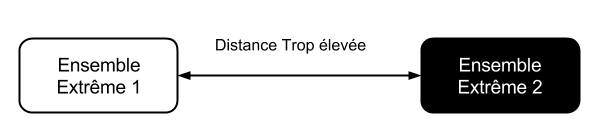
\includegraphics[width=\textwidth]{data/tests/test-coherence-fosse.png}
\caption{Schéma de principe du test de cohérence.}
\end{figure}

Après avoir généré ces deux ensemble de morceaux, il suffit de générer une
playlist avec la base de donnée résultante. Si des morceaux des deux ensembles
sont dans la playlist la qualité de la similarité est à revoir.

Il est important de noter que la taille de la playlist générée est importante,
ainsi que le rang du premier morceau non valide. En effet, plus la playlist est
grande, plus le risque de traverser le fossé est grand. On fixera donc la taille
de la playlist à générer à 1000 morceaux, ce qui est largement suffisant pour
tester la robustesse de la similarité (la plupart des playlists générées ne
dépassant pas 100 pistes). De plus, un morceau non valide à un rang élevé (par
exemple la 800e piste) est moins critique pour la qualité de la playlist qu'un
rang bas (par exemple 10e piste).

Il faut donc prendre en compte ces éléments dans la mise en place d'un score de
réussite au test. On calculera ce score en fonction du rang du morceau non
valide dans la playlist. Une playlist sans morceau invalide aura un score de
100\%.

On utilise donc la formule suivante pour calculer le score du test, n
correspondant au rang de la piste invalide, et N à la taille de la playlist
générée (généralement 1000)~:

\begin{equation*}
  score(n) = log_{10}(1 + \frac{n}{N} * 9)
\end{equation*}

Grâce à cette formule, le score atteint 70\% à la moitié de la playlist (500).
Ainsi les premier rang sont plus important pour le score que les derniers.

En réalisant ce test de multiples fois et en faisant la moyenne des scores
obtenus on obtient un aperçu assez clair de la qualité de la cohérence induite
par notre calcul de similarité.

\subsection{Test de variation : Technique de la «~Passerelle~»}
\label{tests:qualite:variation-passerelle}

Ce test permet de tester la \emph{variation} de la playlist. Pour cela il
utilise les deux ensembles extrêmes utilisés par le test de cohérence, en 
ajoutant un troisième ensemble qui jouera le rôle de passerelle entre les
deux autres.

L'ensemble passerelle sera généré pour contenir des morceaux qui comblent le
vide entre les deux ensembles extrêmes~:

\begin{itemize}
  \item rythme entre 0.2 et 0.75
  \item énergie entre 0.35 et 0.85
\end{itemize}

\begin{figure}[H]
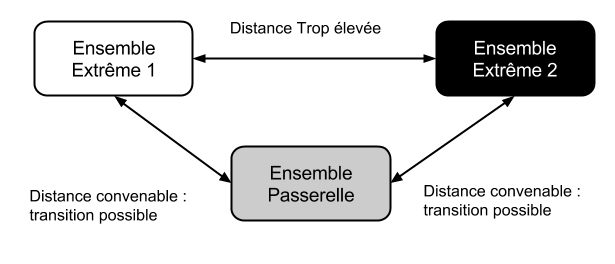
\includegraphics[width=\textwidth]{data/tests/test-variation-passerelle.png}
\caption{Schéma de principe du test de variation.}
\end{figure}

Tout l'enjeu du test est qu'une playlist qui commence par un morceau du premier
ensemble extrême contienne un morceau de l'autre ensemble extrême, le troisième
ensemble servant de pont, grâce à la variation introduite dans le calcul de
similarité.

Pour que le test soit viable, l'ensemble passerelle doit être construit de
manière réfléchie~: la distance entre les morceaux la composant doit être faible,
il ne faut pas qu'il y ait de discontinuité dans les descripteurs, sinon la
passerelle ne marchera pas.

Comme pour le test de cohérence on génère des playlists de 1000 morceaux.
Cependant, cette fois ci le score doit prendre en compte deux événements~:
\begin{description}
  \item[Le rang du premier morceau de la passerelle~:] car c'est la première
  étape, un algorithme de similarité qui n'arrive pas à ce stade prend très peu
  en charge la variation.
  \item[Le rang du premier morceau de l'autre ensemble extrême~:] c'est
  l'aboutissement du test. Il est important de noter qu'un rang trop bas indique
  Un manque de cohérence pour la similarité.
\end{description}

Le meilleur moyen de conduire ce test est encore une fois de le répéter. On
obtiens ainsi une moyenne des rangs d'atteinte de la passerelle et de ceux
d'atteinte de l'autre extrême.

\subsection{Test de comparaison de similarité}
\label{tests:qualite:comparaison}

Ce test vise a fournir une visualisation des variations de comparaisons entre
les morceaux d'une playlist générée. Tout d'abord, on génère une playlist grâce
au générateur. On compare les morceaux de la façon suivante~: on calcule la
similarité entre une piste (indice $k$) et la piste suivante (indice $k+1$),
et on la compare à la similarité entre la piste au n-ième rang précédent
(indice $k-n$) et la piste suivante (indice $k+1$). Ce qui nous donne la
formule suivante ($\Delta{}sim_{n}$ étant la différence de similarité pour un
rang n)~:

\begin{itemize}
  \item $n \in \mathbb{N}^{*}$, le rang du morceau précédent.
  \item $k \in \mathbb{N}$ et $k \geq n$
  \item $T_{k}$ designant le k-ième morceau de la playlist.
\end{itemize}

\begin{equation*}
  \Delta{}sim_{n}(k) = |sim(T_{k-n}, T_{k+1}) - sim(T_{k}, T_{k+1})|
\end{equation*}

En faisant varier le rang n on peut observer les variation pour des morceaux
plus éloignés. Un rang de 1 comparera la piste courante avec la piste la
précédant.

\begin{figure}[H]
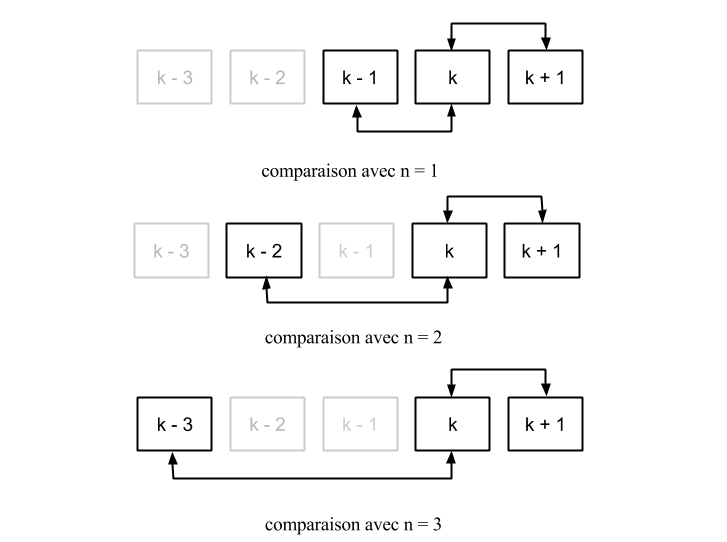
\includegraphics[width=\textwidth]{data/tests/test-comparaison.png}
\caption{Illustration du système de comparaison pour différentes valeurs de n}
\end{figure}

Avec les résultats de cette fonction de comparaison, on peut calculer la
distance de similarité pour tout k. On obtient donc ainsi un graphe, construit
avec GNUPlot par exemple, qui nous montre les variations de similarité. Ce
graphe permet de visualiser les mauvais enchaînements de morceaux, car la valeur
de la fonction $\Delta{}sim_{n}$ sera élevée lors de ces transitions violentes.
De plus, il est intéressant de superposer plusieurs de ces graphes présentant un
rang n différent. On peut ainsi distinguer à partir de quelle rang la cohérence
disparaît.
